\documentclass[german]{../spicker}

\usepackage{amsmath}

\usepackage{graphicx}
\usepackage{tabularx, multirow}

\title{IT-Grundlagen}
\author{Patrick Gustav Blaneck}
\makeindex[intoc]
\makeindex[intoc, name=Beispiele,title=Beispiele]

\newcommand{\scalarprod}[1]{\left\langle #1 \right\rangle}
\newcommand{\vektor}[1]{\begin{pmatrix*}[r] #1 \end{pmatrix*}}
\renewcommand{\span}[1]{\operatorname{span}\left(#1\right)}
\newcommand{\dx}{~\mathrm{d}x}

\newenvironment{allintypewriter}{\ttfamily}{\par}
\newcommand*{\ditto}{\texttt{\char`\"}}

\begin{document}
\maketitle
In dieser Zusammenfassung werden Inhalte aus dem ITG-Skript von Bastian Küppers verwendet.
\tableofcontents
\newpage

%\setcounter{section}{1}

\section{Codierung}
\subsection{Stellenwertsysteme}

\begin{defi}{Stellenwertsystem}
    Allgemein lässt sich der Wert einer Zahl in einem Stellenwertsystem zur Basis $B$ wie folgt ausdrücken ($d_i$ ist der Wert der $i$-ten Stelle, $r$ der Exponent der höchtswertigen Stelle):
    $$
        n_b = \sum^r_{i=0} B^i \cdot d_i
    $$
\end{defi}

\begin{algo}{Dezimal $\to$ Binär, Hexadezimal, $\ldots$}
    Sei $B = 2$ für Umrechnung ins Binärsystem, bzw. $B =16$ für das Hexadezimalsystem.

    Es gilt für eine umzurechnende Zahl $z$:

    $$
        \begin{aligned}
            z : B       & = z_0 \quad     &  & \text{Rest } r_0     \\
            z_0 : B     & = z_1 \quad     &  & \text{Rest } r_1     \\
            z_1 : B     & = z_2 \quad     &  & \text{Rest } r_2     \\
                        & \ldots          &  &                      \\
            z_{n-2} : B & = z_{n-1} \quad &  & \text{Rest } r_{n-1} \\
            z_{n-1} : B & = 0 \quad       &  & \text{Rest } r_n
        \end{aligned}
    $$

    Damit gilt dann: $(z)_{10} = (r_nr_{n-1}\ldots r_2r_1r_0)_B$ (also gelesen von \emph{unten nach oben}).\qed
\end{algo}

\begin{algo}{Binär $\to$ Hexadezimal}
    Sei eine Binärzahl $b$ gegeben mit $n \in 4\N$ Bits.

    Dann kann $b$ wie folgt in eine Hexadezimalzahl $h$ mit $m = \frac{n}{4}$ Zeichen umgeformt werden:

    $$
        \underbrace{b_{n-1}b_{n-2}b_{n-3}b_{n-4}}_{h_{m-1}} ~ \ldots ~ \underbrace{b_7b_6b_5b_4}_{h_1} ~ \underbrace{b_3b_2b_1b_0}_{h_0}
    $$

    Erinnerung: 4 Bits können binär nur 16 mögliche Werte annehmen!
\end{algo}

\newpage
\subsection{Zahlendarstellungen}

\begin{defi}{Einerkomplement}
    Das \emph{Einerkomplement} einer Binärzahl wird gebildet, indem man alle Bits negiert.

    Das erste Bit gibt dabei das Vorzeichen an.

    Nachteile: Doppelte Darstellung der Null, Subtraktion lässt sich nicht auf Addition mit einer negativen Zahl zurückführen
\end{defi}

\begin{defi}{Zweierkomplement}
    Das \emph{Zweierkomplement} einer Binärzahl wird gebildet, indem man das Einerkomplement bildet und zusätzlich $1$ addiert.

    Das erste Bit gibt dabei das Vorzeichen an.

    Vorteile: Subtraktion entspricht Addition mit einer negativen Zahl, keine doppelte Null
\end{defi}

\begin{defi}{Binäre Festkommazahlen}
    Die Umwandlung des ganzzahligen Anteils einer (dezimalen) Festkommazahl erfolgt analog zu ganzen Zahlen.

    Zusätzlich werden aber die Nachkommastellen mit entsprechend negativen Exponenten weiter \glqq verrechnet\grqq.
\end{defi}

\begin{defi}{Gleitkommazahlen nach \emph{IEEE 754}}
    Die Darstellung einer Gleitkommazahl
    $$
        x = s \cdot m \cdot b^e
    $$
    besteht aus
    \begin{itemize}
        \item Vorzeichen $s$ (1 Bit)
        \item Mantisse $m$ ($p$ Bits, $p_{\text{float}} = 23$, $p_{\text{double}} = 52$)
        \item Basis $b$ (bei normalisierten Gleitkommazahlen nach IEEE ist $b = 2$)
        \item Exponent $e$ ($r$ Bits, $r_{\text{float}} = 8$, $r_{\text{double}} = 11$)
    \end{itemize}
\end{defi}

\begin{algo}{Umrechnung in \emph{IEEE 754}}
    \begin{itemize}
        \item Umwandeln einer Dezimalzahl in eine \emph{binäre Festkommazahl} ohne Vorzeichen.
        \item Normalisieren der \emph{Mantisse}:\\
              Das Komma wird $n$ Stellen nach links verschoben, so dass dort nur noch eine 1 als ganzzahliger Anteil vorhanden ist. ($n$ ist bei Verschieben nach rechts negativ!)\\
              $M$ ist dann der \emph{Nachkommateil}.
        \item Bestimmen des \emph{Exponenten}: $E = (\text{bias } + n)_2$ (bias ist meist $127$, wenn nicht anders gegeben)
        \item Bestimmen des \emph{Vorzeichenbits} $s$
        \item Zusammensetzen der Gleitkommazahl
              $$
                  s \mid E \mid M
              $$
    \end{itemize}
\end{algo}

\subsection{Zeichendarstellungen}

\begin{defi}{UTF-8 Codierung}
    \begin{tabular}{| c | r | c |}
        \hline
        Unicode-Bereich       & \multicolumn{1}{|c|}{UTF-8-Codierung}   & Möglichkeiten        \\
        \hline
        0000 0000 - 0000 007F & 0xxx xxxx                               & 128 (7 Bits)         \\
        0000 0080 - 0000 07FF & 110x xxxx 10xx xxxx                     & 2.048 (11 Bits)      \\
        0000 0800 - 0000 FFFF & 1110 xxxx 10xx xxxx 10xx xxxx           & 65.536  (16 Bits)    \\
        0001 0000 - 0010 FFFF & 1111 0xxx 10xx xxxx 10xx xxxx 10xx xxxx & 2.097.152  (21 Bits) \\
        \hline
    \end{tabular}
\end{defi}

\subsection{Spezielle Codierungen}

\begin{algo}{Huffman-Codierung}
    \begin{enumerate}
        \item Schreibe Buchstaben mit Auftrittshäufigkeiten als \glqq Wald\grqq.
        \item Fasse die beiden Bäume mit der geringsten Auftrittshäufigkeiten zu einem neuen Baum zusammen, dabei werden die Auftrittshäufigkeiten addiert.
        \item Wiederhole, bis nur noch ein Baum existiert.
        \item Codierung eines Buchstaben entspricht dann dem \emph{Pfad} zum entsprechenden Blatt mit \glqq links\grqq $\to$ 0, \glqq rechts\grqq $\to$ 1
    \end{enumerate}

    Mittlere Codelänge:
    $$
        L(C) = \frac{\#\text{Bits der verschlüsselten Nachricht}}{\#{\text{Zeichen der verschlüsselten Nachricht}}}
    $$
\end{algo}

\begin{defi}{Hamming-Codierung}
    Bei der Hamming-Codierung werden Paritätsinformationen zu Daten hinzugefügt, um so mögliche Übertragungsfehler zu erkennen.

    Hamming-Codewörter haben die Länge $N = 2^k-1$, wobei $k$ Paritätsbits enthalten sind.
    Die Bits werden der Einfachheit halber bei Eins beginnend durchnummeriert.
    Die Paritätsbits stehen an den Stellen, deren Index eine 2er-Potenz ist.

    Sind $p_1, p_2, \ldots, p_k$ Paritätsbits, $d_1, d_2, \ldots, d_{N-k}$ Bits des Datenwortes und $c_1, c_2, \ldots, c_N$ die Bits des zu bildenden Codewortes, hat ein Codewort des so konstruierten Hamming-Codes die folgende Form:

    \begin{tabular}{| c | c | c || c | c | c | c || c | c | c | c | c | c | c | c || c | c | c |}
        \hline
        $c_1$ & $c_2$ & $c_3$ & $c_4$ & $c_5$ & $c_6$ & $c_7$ & $c_8$ & $c_9$ & $c_{10}$ & $c_{11}$ & $c_{12}$ & $c_{13}$ & $c_{14}$ & $c_{15}$ & $c_{16}$ & $c_{17}$ & \ldots \\
        \hline
        $p_0$ & $p_1$ & $d_1$ & $p_2$ & $d_2$ & $d_3$ & $d_4$ & $p_3$ & $d_5$ & $d_6$    & $d_7$    & $d_8$    & $d_9$    & $d_{10}$ & $d_{11}$ & $p_4$    & $d_{12}$ & \ldots \\
        \hline
    \end{tabular}\\

    Dabei wird jedem Paritätsbit eine spezielle Bitmaske zugewiesen:

    \begin{tabular}{| c || c | c | c || c | c | c | c || c | c | c | c | c | c | c | c || c |}
        \hline
                       & $c_1$ & $c_2$ & $c_3$ & $c_4$ & $c_5$ & $c_6$ & $c_7$ & $c_8$ & $c_9$ & $c_{10}$ & $c_{11}$ & $c_{12}$ & $c_{13}$ & $c_{14}$ & $c_{15}$ & \ldots \\
        \hline
        Bitmaske $p_0$ & $p_0$ & $p_1$ & 1     & $p_2$ & 1     & 0     & 1     & $p_3$ & 1     & 0        & 1        & 0        & 1        & 0        & 1        & \ldots \\
        Bitmaske $p_1$ & $p_0$ & $p_1$ & 1     & $p_2$ & 0     & 1     & 1     & $p_3$ & 0     & 1        & 1        & 0        & 0        & 1        & 1        & \ldots \\
        Bitmaske $p_2$ & $p_0$ & $p_1$ & 0     & $p_2$ & 1     & 1     & 1     & $p_3$ & 0     & 0        & 0        & 1        & 1        & 1        & 1        & \ldots \\
        Bitmaske $p_3$ & $p_0$ & $p_1$ & 0     & $p_2$ & 0     & 0     & 0     & $p_3$ & 1     & 1        & 1        & 1        & 1        & 1        & 1        & \ldots \\
        \hline
    \end{tabular}\\

    Damit gilt:
    $$
        \begin{aligned}
            c_1 = p_0 & = c_3 \oplus c_5 \oplus c_7 \oplus c_9 \oplus c_{11} \oplus c_{13} \oplus c_{15} \oplus \ldots    \\
                      & \iff \text{jedes ungerade Datenbit}                                                               \\
            c_2 = p_1 & = c_3 \oplus c_6 \oplus c_7 \oplus c_{10} \oplus c_{11} \oplus c_{14} \oplus c_{15} \oplus \ldots \\
                      & \iff \text{ein Datenbit rechts von $p_1$, zwei überspringen, zwei einberechnen, $\ldots$}         \\
            c_4 = p_2 & = c_5 \oplus c_6 \oplus c_7 \oplus c_{12} \oplus c_{13} \oplus c_{14} \oplus c_{15} \oplus \ldots \\
                      & \iff \text{drei Datenbit rechts von $p_2$, vier überspringen, vier einberechnen, $\ldots$}
        \end{aligned}
    $$
\end{defi}

\begin{algo}{Fehlererkennung beim Hamming-Code}
    Situation: Empfangen eines Hamming-codierten Datensatzes

    \begin{enumerate}
        \item Erneutes Berechnen der \emph{Paritätsbits}
        \item Erkennen, welche neu berechneten Paritätsbits $p'_i$ \emph{verschieden} sind zu den empfangenen Paritätsbits $p_i$
        \item Bitfehler ist in dem Datenbit passiert, in dem gilt:
              \subitem $p_i = p'_i \implies$ Bitmaske für $p_i$ ist $0$
              \subitem $p_i \neq p'_i \implies$ Bitmaske für $p_i$ ist $1$
    \end{enumerate}

    Es wird angenommen, dass nur ein Bitfehler in den Datenbits passiert ist.

    Anmerkung: Ist lediglich ein Paritätsbit verschieden, dann ist ein Übertragungsfehler in dem betreffenden Paritätsbit selbst aufgetreten, da alle Datenbits zur Berechnung von mindestens zwei Paritätsbits verwendet werden.
\end{algo}

\section{Formale Sprachen}
\subsection{Backus-Naur-Form}

\begin{defi}{(kontextfreie) Grammatik}
    Eine (kontextfreie) Grammatik $G$ ist ein 4-Tupel $\{N, T, \Sigma, P\}$ mit folgenden Eigenschaften:
    \begin{itemize}
        \item $N$ ist eine endliche Menge von \emph{Nichtterminalsymbolen},
        \item $T$ ist eine endliche Menge von \emph{Terminalsymbolen},
        \item ein \emph{Startsymbol} $\Sigma \in N$,
        \item eine endliche Menge an Produktionsregeln $P \subset N \times T^*$.
    \end{itemize}
    Es gilt $N \cap M = \emptyset$. $^*$ bezeichnet die Kleensche Hülle.

    Anmerkung: Die Notation verhält sich in der Vorlesung sehr anders als in den meisten Quellen.
\end{defi}

\begin{defi}{Backus-Naur-Form}
    In der \emph{Backus-Naur-Form} werden Symbole durch eine Zuweisung definiert.\\
    Diese wird durch den Operator \texttt{:=} dargestellt.

    \begin{itemize}
        \item Dabei gilt weiterhin, dass in der Zuweisung eines \emph{Nichtterminalsymbols} mindestens ein weiteres Symbol auftauchen muss und
        \item bei der Zuweisung eines \emph{Terminalsymbols} nur Zeichen des Alphabets.
        \item Bei einer Zuweisung können mehrere Symbole oder Zeichen(-ketten) des Alphabets verbunden werden.
        \item Durch ein Leerzeichen (\glqq ~~~\grqq, \texttt{space}) wird eine \texttt{und}-Verknüpfung definiert,
        \item durch einen senkrechten Stricht (\glqq ~$\mid$~\grqq, \texttt{pipe}) wird eine \texttt{oder}-Zuweisung definiert.
        \item Zur logischen Gliederung der Verknüpfungen können Klammern verwendet werden.
        \item Es ist ebenfalls möglich Kardinalitäten für Symbole zu definieren:
              \subitem Geschweifte Klammern \texttt{\{\}} definieren dabei eine \emph{beliebige Wiederholung} und
              \subitem eckige Klammern \texttt{[]} definieren ein \emph{einmaliges Auftreten}.
              \subitem In beiden Fällen ist das Weglassen des Symbols ebenfalls möglich.
    \end{itemize}
\end{defi}

\begin{example}{Backus-Naur-Form}
    \begin{allintypewriter}
        \begin{tabular}{rl}
            Satz        & := Subjekt Verb Präposition Nomen Ende                       \\
            Subjekt     & := Nomen                                                     \\
            Nomen       & := Artikel Substantiv                                        \\
            Artikel     & := \ditto der\ditto | \ditto die\ditto | \ditto das\ditto    \\
            Substantiv  & := \ditto Mann\ditto | \ditto Frau\ditto | \ditto Haus\ditto \\
            Verb        & := \ditto geht\ditto                                         \\
            Präposition & := \ditto in\ditto                                           \\
            Ende        & := \ditto .\ditto
        \end{tabular}
    \end{allintypewriter}
\end{example}

\subsection{Programmiersprachen}

\begin{defi}{Compiler}
    Das Programm, welches den
    menschenlesbaren \emph{Quellcode} anhand der Regeln der zugrundeliegenden Grammatik
    interpretiert und in maschinenlesbare Anweisungen überführt, wird \emph{Compiler} genannt.

    Die maschinenlesbaren Anweisungen können dabei entweder direkt in eine
    maschinenspezifische Binärfolge umgewandelt werden, oder in einen sogenannten
    \emph{Bytecode}.

    Im zweiten Fall kann der Bytecode,
    auch Zwischencode genannt, noch an beliebigen Prozessortypen angepasst werden,
    muss dafür aber vor der Ausführung erneut bearbeitet werden.

    Bei der Kompilierung eines Programms werden zwei Phasen durchlaufen:
    \begin{enumerate}
        \item \textbf{Analysephase}, in der der Quellcode analysiert und auf Fehler geprüft wird:
              \subitem \underline{\emph{Lexer} (lexikalischer Scanner)}: \\
              Quellcode wird in einzelne Teile (\emph{Tokens}) zerlegt und klassifiziert (z.B. als \emph{Schlüsselwörter} oder \emph{Bezeichner}).\\
              Der Lexer erkennt hier z.B. falsch benannte Variablen.
              \subitem \underline{\emph{Parser} (syntaktische Analyse)}: \\
              Vom Lexer erzeugte \emph{Tokens} werden dem \emph{Parser} übergeben.
              Der Parser überprüft den Quellcode auf Fehler und setzt ihn bei Fehlerfreiheit in einen \emph{Syntaxbaum} (AST) um.\\
              Hier werden Fehler wie fehlende Semikolons oder falsche genutzte Operatoren erkannt.
              \subitem \underline{\emph{Semantische Analyse}}: \\
              Hier wird z.B. kontrolliert, ob eine verwendete Variable auch vorher deklariert wurde, oder ob Quell- und Zieltyp einer Anweisung übereinstimmen. Dabei erzeugte Metadaten werden in den AST integriert.
              In diesem Schritt werden generell semantische Fehler erkannt, d.h. Anweisungen, die korrekt aussehen, aber fehlerhaft sind.
              \\
        \item \textbf{Synthesephase}, in der Binär- bzw. Bytecode erzeugt wird:
              \subitem \underline{\emph{Zwischencodeerzeugung}}: \\
              Hier wird plattformunabhängiger Bytecode erzeugt, der als Grundlage für den nächsten Schritt dient.
              \subitem \underline{\emph{Optimierung}}: \\
              Während der Optimierung wird versucht die Performanz des erzeugten Programms zu steigern.
              \subitem \underline{\emph{Codegenerierung}}: \\
              Hier wird aus dem optimierten Zwischencode der \emph{Binärcode} erzeugt.
    \end{enumerate}
\end{defi}

\begin{bonus}{Ahead-of-Time Compiler}
    Bei dieser Variante wird der gesamte Quellcode \emph{in einem Rutsch}
    in Binär- oder Bytecode übersetzt. Das kann mitunter dazu führen, dass die Kompilierung
    sehr lange dauert.
\end{bonus}

\begin{bonus}{Just-in-Time Compiler}
    Daher haben sich mit der Zeit auch sogenannte \emph{Just-in-
        Time Compiler} etablieren können, die nur einen kleinen Teil des Quellcodes direkt
    übersetzen und weitere Teile des Quellcodes erst dann übersetzen, \emph{wenn sie bei der
        Programmausführung benötigt werden}.
\end{bonus}

\begin{defi}{Linker}
    Nachdem der Compiler den Binärcode erzeugt hat, muss der \emph{Linker} daraus noch
    ein lauffähiges Programm erstellen. Das ist insbesondere der Fall, wenn es mehrere
    Dateien mit Quellcode gibt.

    Dies geschieht indem der Binärcode zu den verschiedenen
    Quellcodedateien, der nun in sogenannten \emph{Objektdateien} vorliegt, zusammengefügt wird. Dabei werden beispielsweise symbolische Adressen aus mehreren
    Quellcodemodulen und externen Bibliotheken so angepasst, dass sie zusammen
    passen.

    Dabei wird zwischen \emph{statischem Linken} und \emph{dynamischen Linken} unterschieden:

    Beim \textbf{statischen Linken} werden alle verfügbaren Objektdateien zu \emph{einer
        einzigen, ausführbaren Programmdatei} gelinkt.
    \begin{itemize}
        \item Vorteil: keine externen Abhängigkeiten, Programm auf jedem geeigneten System ohne Weiteres lauffähig
        \item Nachteil: nicht mehr möglich, einzelne Programmteile auszutauschen ohne den Linkvorgang vollständig zu wiederholen,
    \end{itemize}
    Beim \textbf{dynamischen Linken} werden Funktions- und Variablenadressen erst zur Laufzeit aufgelöst, sodass externe Bibliotheken
    einfach in Form von \emph{Dynamically Linked Libraries} (DLLs) bzw. \emph{Shared Objects} (SOs) angesprochen werden können. Da DLLs bzw. SOs als existierend
    vorausgesetzt werden, wird das fertige Programm bei dynamischem Linken kleiner.
    \begin{itemize}
        \item Vorteil: mehrere Programme können dieselbe externe Bibliothek verwenden, ohne dass der benötigte Code mehrfach in einzelne Programme integriert werden muss.
    \end{itemize}
\end{defi}

\begin{defi}{Interpreter}
    \emph{Interpreter} zeichnen sich dadurch aus, dass der Quellcode nicht einmalig in Binärcode übersetzt wird, sondern bei jeder Programmausführung schrittweise abgearbeitet wird.
    \begin{itemize}
        \item Vorteile: einfache Portabilität, dynamischere Quellcodeverwaltung
        \item Nachteile: deutlich langsamere Ausführungsgeschwindigkeit, keine Optimierungen an Programmstruktur möglich
    \end{itemize}
\end{defi}

\section{Rechnerarchitekturen}
\subsection{Von-Neumann-Architektur}

\begin{defi}{Von-Neumann-Architektur}
    Im Grundsatz besteht die Architektur aus drei Komponenten: \emph{CPU}, \emph{Speicher} und \emph{I/O Einheit}.

    Die einzelnen Komponenten sind über Datenleitungen, sogenannte \emph{Busse}, verbunden.
    \begin{center}
        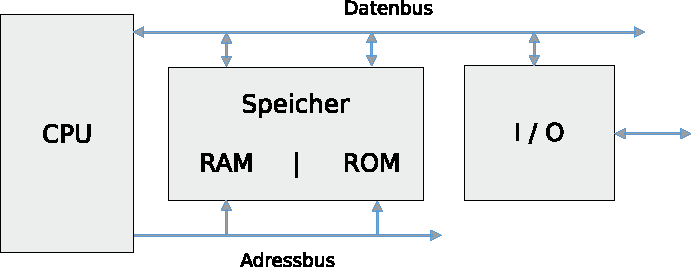
\includegraphics[]{images/von_neumann.pdf}
    \end{center}
\end{defi}

\begin{defi}{CPU}
    Die \emph{CPU} (\emph{Central Processing Unit}, Prozessor) ist sozusagen das Gehirn des Computers.
    Die CPU besteht im Wesentlichen aus drei Teilen, dem \emph{Leitwerk} und
    dem \emph{Rechenwerk} und den \emph{Registern}, welche direkt zur Abarbeitung von Befehlen
    benötigte Daten und berechnete Ergebnisse aufnehmen können.

    Das \emph{Leitwerk} steuert die Ausführung des Binärcodes, das \emph{Rechenwerk} führt anfallende Rechenoperationen aus.
\end{defi}

\begin{bonus}{Aufbau Rechenoperationen}
    \begin{itemize}
        \item \emph{Operationsteil}: codiert konkreten Befehl
        \item \emph{Operanden}: stellen z.B. Summanden einer Operation, oder Adresse einer Variablen dar
    \end{itemize}
\end{bonus}

\begin{bonus}{Abarbeitung von Befehlen}
    Jeder Befehl durchläuft bei der Abarbeitung in der CPU folgende Schritte:
    \begin{itemize}
        \item \emph{Instruction Fetch (IF)} : Befehl lesen
        \item \emph{Instruction Decode (ID)} : Befehl decodieren
        \item \emph{Fetch Operands (FO)} : Operanden laden
        \item \emph{Execute (EX)} : Befehl ausführen
        \item \emph{Writeback (WB)} : Ergebnis schreiben
    \end{itemize}

    \begin{center}
        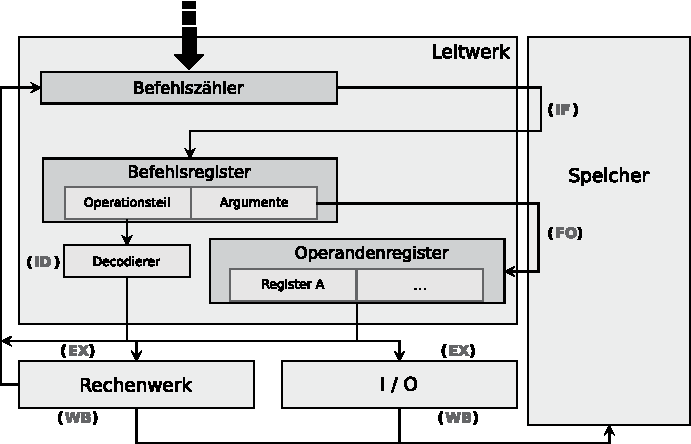
\includegraphics[]{images/befehlsabarbeitung.pdf}
    \end{center}
\end{bonus}

\begin{defi}{Prozessorarchitekturen}
    \textbf{CISC} (\emph{Complex Instruction Set Computer}):\\
    Eine CISC CPU zeichnet sich durch einen \emph{komplexen Befehlssatz} in Form von \emph{Microcode} und dem Vorhandensein nur \emph{weniger Register} aus.

    \textbf{RISC} (\emph{Reduced Instruction Set Computer}):\\
    eine RISC CPU nur über \emph{wenige, in Hardware realisierte Befehle} und \emph{viele Prozessorregister}.
\end{defi}

\begin{defi}{Pipelining}
    In einer \emph{RISC CPU}, die nur wenige und elementare Befehle verwendet, kann dafür
    gesorgt werden, dass alle Teilschritte, deren \emph{parallele Verarbeitung} das Pipelining
    ermöglicht, gleich lange dauern. Nur deswegen kann das Konzept des Pipelinings
    erfolgreich umgesetzt werden.

    Das ist bei einer \emph{CISC CPU} aufgrund der vielen
    und teils sehr komplexen Befehle \emph{nicht} möglich.
\end{defi}

\begin{example}{Pipelining}
    5-Stage-Pipeline:
    \begin{itemize}
        \item Instruction Fetch (\textbf{IF}): Befehl lesen
        \item Instruction Decode (\textbf{ID}) : Befehl decodieren
        \item Execute (\textbf{EX}) : Ausführen
        \item Memory Access (\textbf{MEM}) : Ausführen
        \item Writeback (\textbf{WB}) : Ergebnis schreiben
    \end{itemize}

    \begin{center}
        \begin{tabular}{| c || m{0.05\textwidth} | m{0.05\textwidth} | m{0.05\textwidth} | m{0.05\textwidth} | m{0.05\textwidth} | m{0.05\textwidth} |}
            \hline
            Instr. 1    & \texttt{IF}            & \texttt{ID}            & \texttt{EX}            & \texttt{MEM}           & \texttt{WB}            &                        \\
            \hline
            Instr. 2    &                        & \texttt{IF}            & \texttt{ID}            & \texttt{EX}            & \texttt{MEM}           & \texttt{WB}            \\
            \hline
            Instr. 3    &                        &                        & \texttt{IF}            & \texttt{ID}            & \texttt{EX}            & \texttt{MEM}           \\
            \hline
            Instr. 4    &                        &                        &                        & \texttt{IF}            & \texttt{ID}            & \texttt{EX}            \\
            \hline
            Instr. 5    &                        &                        &                        &                        & \texttt{IF}            & \texttt{ID}            \\
            \hline
            \hline
            Clock Cycle & \multicolumn{1}{c|}{1} & \multicolumn{1}{c|}{2} & \multicolumn{1}{c|}{3} & \multicolumn{1}{c|}{4} & \multicolumn{1}{c|}{5} & \multicolumn{1}{c|}{6} \\
            \hline
        \end{tabular}
    \end{center}
\end{example}

\begin{defi}{ROM}
    Der \emph{ROM} ist ein Festwertspeicher, der - prinzipiell - \emph{nur gelesen} werden kann und die Firmware des Computers gespeichert hat.

    Im ROM liegt das sogenannte \emph{BIOS} (\emph{basic input output system}) bzw. moderner \emph{UEFI}
    (\emph{unified extensible firmware interface}).
    Die im ROM abgelegten Informationen stellen die Firmware des
    Rechners dar. Diese Firmware sorgt dafür, dass der Computer nach dem Einschalten
    in die Lage versetzt wird, grundlegende Hardwarekomponenten zu verwalten.
\end{defi}

\begin{defi}{RAM}
    Der \emph{RAM},
    auch \emph{Hauptspeicher} genannt, ist ein Speicher mit \emph{wahlfreiem Zugriff}, der seinen
    Inhalt jedoch bei Verlust der Betriebsspannung \emph{verliert}. Im RAM werden Informationen
    abgelegt, die ein \emph{Programm zur Laufzeit} benötigt.

    Sollen Daten
    über das Ende des Programms hinaus gespeichert werden, müssen sie über die
    \emph{I/O-Einheit} auf einen anderen Speicher geschrieben werden.
\end{defi}

\begin{defi}{Cache}
    \emph{Cache} ist \emph{schneller} als RAM, kann aber nur \emph{weniger Speicherkapazität} zur Verfügung stellen.

    Das bedeutet, dass der Cache nur kleine Datenmengen, sogenannte \emph{Cacheblocks}, aus dem Hauptspeicher vorhalten kann.
    Diese haben eine definierte Größe und können dann schneller in die CPU geldaden werden, als das aus dem RAM möglich wäre.
\end{defi}

\begin{defi}{Lokalität}
    \textbf{Zeitliche Lokalität}:\\
    Es ist, bei entsprechender Programmierung, sehr wahrscheinlich, dass
    auf eine Speicherzelle nicht nur einmal, sondern in kurzer Zeit \emph{mehrmals zugegriffen}
    wird.

    \textbf{Örtliche Lokalität}:\\
    Es ist, bei entsprechender Programmierung, sehr wahrscheinlich, dass nach
    dem Zugriff auf eine bestimmte Speicherzelle auch ein \emph{Zugriff in deren unmittelbarer
        \glqq Nachbarschaft\grqq} stattfindet.
\end{defi}

\begin{bonus}{Aufbau eines Caches}
    \begin{center}
        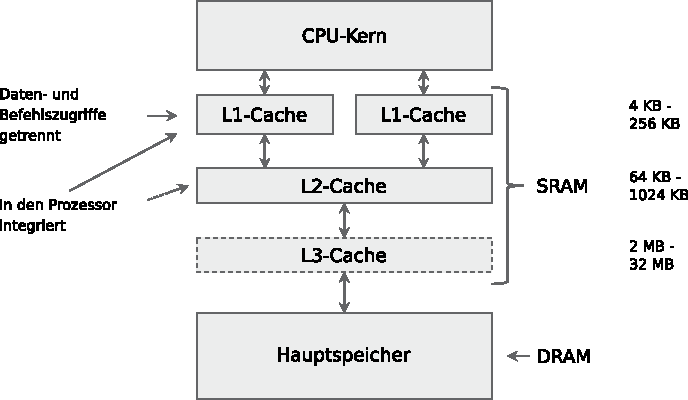
\includegraphics[]{images/cache_aufbau.pdf}
    \end{center}

    Aus der Abbildung ist ersichtlich, dass der Cache selbst ebenenweise organisiert ist.

    Im Regelfall sind mindestens die Ebenen L1 und L2 vorhanden, oftmals sogar noch
    eine dritte Ebene L3. Dabei ist in jedem Fall der L1-Cache in die CPU integriert,
    häufig auch noch der L2-Cache.

    Beginnend beim
    L3-Cache werden die Cachelevel mit größerer Nähe zur CPU jeweils kleiner und
    schneller. Dieser Aufbau soll die Frage nach der Auswahl der Daten, die im Cache
    vorgehalten werden, vereinfachen. Es ist also möglich einen relativ großen Datenbestand
    im L3-Cache vorzuhalten, der schneller ist als der Hauptspeicher. Von dort
    aus kann dann wiederum eine Teilmenge der Daten im noch schnelleren L2-Cache
    vorgehalten werden, usw.

    Liegen benötigte Daten nicht im L1-Cache, welcher Daten bzw. Befehle schlussendlich an die CPU liefert, ist aufgrund der Lokalität und
    des Aufbaus des Caches die Wahrscheinlichkeit hoch, dass die benötigten Daten
    nicht aus dem langsamen Hauptspeicher geladen werden müssen, sondern sich in
    einem der niedrigeren Cache-Level finden und damit immer noch vergleichsweise
    schnell zur Verfügung gestellt werden können.
\end{bonus}

\begin{bonus}{Interner Aufbau eines Cachelevels}
    \begin{center}
        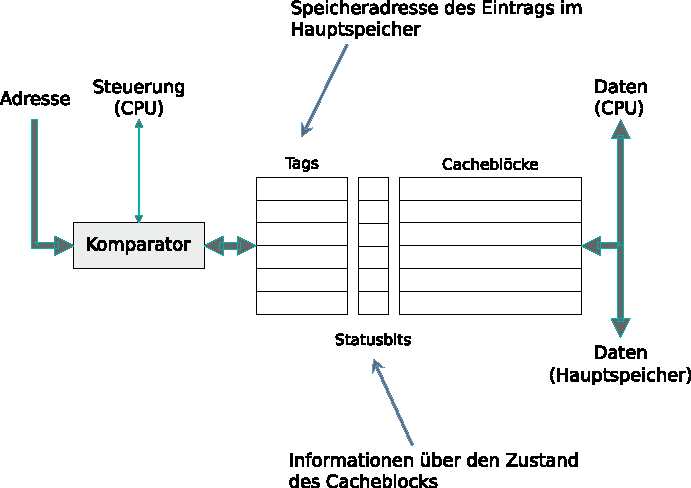
\includegraphics[]{images/cache_level.pdf}
    \end{center}

    Zu jedem Cacheblock wird die Startadresse des Blocks im RAM gespeichert, diese
    Information wird \emph{Tag} genannt.

    Wird von der CPU eine Anfrage an den Speicher
    gestellt, wird zunächst anhand des Tags unter Zuhilfenahme des Komparators geprüft, ob der angefragte Datensatz im Cache liegt. Dabei wird auch geprüft, ob eine
    angefragte Speicheradresse innerhalb eines Cacheblocks liegt. Das ist möglich, da
    der Tag sowie die Größe des Cacheblocks bekannt sind.

    Ist dies nicht der Fall, wird
    die Anfrage an ein niedrigeres Cachelevel bzw. den RAM weitergereicht.

    Außerdem
    werden zu jedem Cacheblock Statusbits gespeichert, die beispielsweise angeben ob
    sich der Cacheblock verändert hat (\emph{dirty bit}), seit er in den Cache geladen wurden,
    oder ob ein Platz im Cache mit einem gültigen Cacheblock belegt ist (\emph{invalid bit}).
\end{bonus}

\begin{defi}{Organisation der Tags}
    Die \emph{Blöcke} (Cache-Lines) eines Caches können in so genannte \emph{Sätze} zusammengefasst werden.
    Für eine bestimmte Adresse ist dann immer nur einer der Sätze zuständig.
    Innerhalb eines \emph{Satzes} bedienen alle Blöcke also nur einen \emph{Teil} aller vorhandenen Adressen.

    Im Folgenden stehe die Variable $m$ für die \emph{Gesamtanzahl der Cacheblöcke} und $n$ für die \emph{Anzahl der Blöcke pro Satz}, die so genannte \emph{Assoziativität}.
    Dann besteht der Cache also aus $\frac {m}{n}$ Sätzen.

    \textbf{Direkt abgebildet} (\emph{DM}, \emph{direct mapped}, $n=1$):\\
    Es gibt pro Cacheblock nur eine einzige Möglichkeit, wo dieser
    platziert werden kann.

    Daher kann es allerdings vorkommen, dass ein Cacheblock
    nicht platziert werden kann, obwohl noch Platz im Cache wäre.

    \textbf{Vollassoziativ} (\emph{FA}, \emph{fully associative}, $n=m$):\\
    Ein Cacheblock kann beliebige auf freie Plätze im Cache zugeordnet
    werden.

    Bei einer Speicheranfrage müssen allerdings alle gespeicherten
    Tags durchsucht werden.

    \textbf{Satzassoziativ} (\emph{SA}, \emph{set associative}, $2\leq n \leq \frac{m}{2}$):\\
    Der verfügbare Platz wird in Gruppen unterteilt. Wie bei einem
    DA Cache gibt es nur eine Gruppe, in der ein Cacheblock platziert werden kann;
    wie bei einem VA Cache kann der Cacheblock innerhalb dieser Gruppe frei platziert
    werden.
\end{defi}

\begin{defi}{Cache-Lesezugriffe}
    Findet ein Lesezugriff auf Speicherzelle $A$ statt, wird geprüft, ob Speicherzelle $A$ bereits im Cache liegt.
    \begin{itemize}
        \item \textbf{$A$ liegt im Cache} (\emph{cache hit}):\\
              Datensatz kann direkt aus dem Cache gelesen werden.
        \item \textbf{$A$ liegt nicht im Cache} (\emph{cache miss}):\\
              Datensatz muss aus dem Hauptspeicher in den Cache geladen werden, danach wird der Datensatz gelesen.
    \end{itemize}
\end{defi}

\begin{defi}{Schreibmodi eines Cache}
    \begin{itemize}
        \item \textbf{write-through} (\emph{WT}):\\
              Datensatz wird im Cache und direkt im Hauptspeicher aktualisiert.

              \emph{Vorteile}: keine Probleme mit Datenkonsistenz im Hauptspeicher\\
              \emph{Nachteile}: hoher Aufwand für Schreiboperationen
        \item \textbf{write-back} (\emph{WB}):\\
              Datensatz wird im Cache aktualisiert und erst dann in den Hauptspeicher geschrieben, wenn der entsprechende Cacheblock aus dem Cache verdrängt wird.

              \emph{Vorteile}: niedrige Belastund der Systembusse, keine Wartezyklen\\
              \emph{Nachteile}: fehlende Datenkonsistenz
    \end{itemize}
\end{defi}

\begin{defi}{Cache-Schreibzugriffe}
    Findet ein Schreibzugriff auf Speicherzelle $A$ statt, wird geprüft, ob Speicherzelle $A$ bereits im Cache liegt.
    \begin{itemize}
        \item \textbf{$A$ liegt im Cache} (\emph{cache hit}):\\
              Datensatz wird im Cache (und im Hauptspeicher) aktualisiert.
        \item \textbf{$A$ liegt nicht im Cache} (\emph{cache miss}):\\
              Datensatz wird im Hauptspeicher geschrieben, Inhalt des Caches wird nicht verändert.
    \end{itemize}
\end{defi}

\begin{defi}{Cache Misses}
    \begin{itemize}
        \item \textbf{Capacity Miss}:
              \subitem - tritt auf, wenn Datensatz bereits im Cache war, aber \emph{bereits verdrängt} wurde
              \subitem (aufgrund mangelnder Kapazität)
              \subitem - hauptsächlich bei VA Caches
        \item \textbf{Compulsory Miss}:
              \subitem - tritt auf, wenn ein Datensatz das \emph{erste Mal} verwendet wird
              \subitem - unabhängig vom Typ des Caches
        \item \textbf{Conflict Miss}:
              \subitem - tritt auf, wenn Datensatz bereits im Cache war, aber \emph{bereits verdrängt} wurde
              \subitem (weil ein anderer Cacheblock an entsprechende Stelle gelagert werden sollte)
              \subitem - vor allem bei DA Caches
    \end{itemize}
\end{defi}

\begin{defi}{RAID}
    \textbf{RAID}: \textbf{R}edundant \textbf{A}rray of \textbf{I}ndependent \textbf{D}isks

    Ein \emph{RAID} besteht aus mindestens zwei Festplatten und zielt auf die \emph{Verbesserung einer Eigenschaft ab}:
    \begin{itemize}
        \item Erhöhung der Ausfallsicherheit
        \item Steigerung der Datentransferrate
        \item Erweiterung der Speicherkapazität
        \item Möglichkeit des Austauschs von Festplatten im laufenden Betrieb
        \item Kostenreduktion durch Einsatz mehrerer kostengünstiger Festplatten
    \end{itemize}
\end{defi}

\begin{defi}{RAID-Level}
    Die genaue Funktionsweise des RAID wird durch das sogenannte \emph{RAID-Level} angegeben.

    \begin{itemize}
        \item \textbf{RAID 0}:
              \subitem - höhere Transferraten durch \emph{Striping}
              \subitem - Daten werden auf mehrere Festplatten verteilt
              \subitem - beim Lesen und Schreiben können mehrere Festplatten parallel verwendet werden
              \subitem \emph{Nachteil}: fällt eine Festplatte aus, sind meist alle Daten verloren
        \item \textbf{RAID 1}:
              \subitem - erhöhte Ausfallsicherheit durch \emph{Mirroring}
              \subitem - Daten in gleicher Weise auf mehrere Festplatten gleichzeitig abgelegt
              \subitem - einzelne Daten \emph{können} auch parallel von mehreren Festplatten gelesen werden
              \subitem \emph{Nachteil}: wird eine Datei gelöscht, wird sie auf allen Platten gelöscht (kein Backup!)
        \item \textbf{RAID 5}:
              \subitem - versucht Vorteile von RAID 0 und RAID 1 zu vereinen
              \subitem - höhere Ausfallsicherheit bei höherer Datentransferrate
              \subitem - besteht aus mindestens drei Festplatten
              \subitem - Verwendet Variante von \emph{Striping}:
              \subsubitem - nicht auf alle $n$ Festplatten verteilt
              \subsubitem - auf allen Festplatten Paritätsinformationen zu Daten auf anderen $n-1$ Platten
              \subsubitem - kann Ausfall einer Festplatte kompensieren
    \end{itemize}


    \begin{center}
        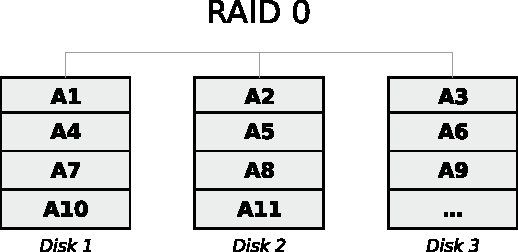
\includegraphics[]{images/raid0.pdf}

        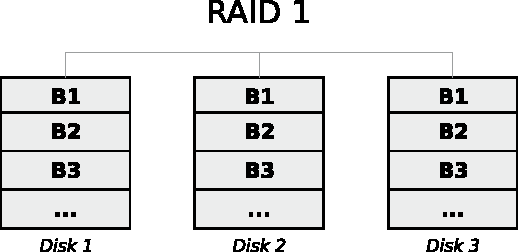
\includegraphics[]{images/raid1.pdf}

        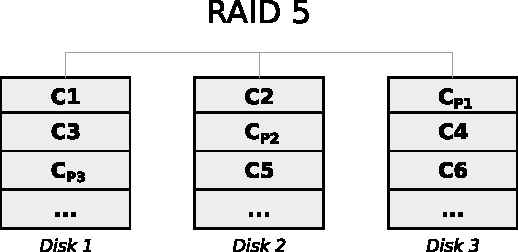
\includegraphics[]{images/raid5.pdf}
    \end{center}

    Merhere RAID-Systeme eines Typs können auch zu einem RAID-System zusammengefasst werden (z.B. \emph{RAID 100}, \emph{RAID 01}, \emph{RAID 10}, \ldots).
\end{defi}

\begin{bonus}{HDD, SSD}
    \textbf{HDD} (Hard Disk Drive, \emph{Festplatte}):
    \begin{itemize}
        \item Gehäuse der Festplatte beinhaltet mehrere, auf einer Achse übereinander montierten, runden Platten, welche mit einer magnetisierbaren Schicht überzogen sind
        \item Schreib-/Leseköpfe werden durch einen zentralen Kamm über die Platten bewegt
        \item \glqq Landing Zone\grqq zum Parken der Köpfe (Berührung $\to$ Datenverlust)
        \item Platten rotieren mit konstanter Umdrehungszahl (5400-15000 rpm)
        \item Kenngrößen:
              \subitem - kontinuierliche Übertragungsrate (\emph{sustained data rate})
              \subitem - mittlere Zugriffszeit (\emph{(data) access time}), bestehend aus:
              \subsubitem - Spurwechselzeit (\emph{seek time})
              \subsubitem - Latenzzeit (\emph{latency})
              \subsubitem - Kommando-Latenz (\emph{controller overhead})
    \end{itemize}


    \textbf{SSD} (Solid State Drive):
    \begin{itemize}
        \item keine mechanischen Bauteile
        \item niedriger Energieverbrauch
        \item hoher Datendurchsatz
        \item hoher Preis pro Speichereinheit
    \end{itemize}
\end{bonus}

\begin{bonus}{Daten- und Adressbus}
    Einzelne Komponenten sind über Leitungen, sogenannte \emph{Busse} verbunden.
    \begin{itemize}
        \item \emph{Datenbus} (bi-direktional)
        \item \emph{Adressbus} (uni-direktional, leitet Adressanfragen der CPU an RAM oder Cache weiter)
    \end{itemize}
\end{bonus}

\subsection{Parallele Rechnerarchitekturen}

\begin{defi}{Flynn'sche Klassifikation (Flynn'sche Taxonomie)}
    \begin{center}
        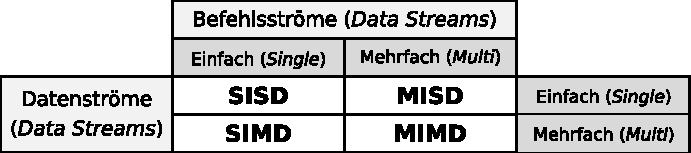
\includegraphics[]{images/flynn.pdf}
    \end{center}

    \begin{itemize}
        \item \emph{SISD} entspricht der Von-Neumann-Architektur
        \item \emph{MIMD} entspricht dem heutigen Mehrprozessorsystem
        \item \emph{SIMD} entspricht dem Aufbau einer Grafikkarte (genutzt in HPC)
        \item \emph{MISD} eher ungebräuchlich.
    \end{itemize}
\end{defi}

\begin{defi}{Shared-Memory Systeme}
    Ein \emph{Shared-Memory System} teilt den vorhandenen RAM unter den verfügbaren Prozessorenkernen auf.
    Das bedeutet, dass Daten zwischen den einzelnen Prozessorkernen \emph{implizit über den RAM} verteilt werden können, da
    jeder Kern Zugriff auf den RAM hat.

    \textbf{SMP} (\emph{symmetric multi processing}) skaliert vergleichweise schlecht.
    Das liegt daran, dass an die vorhandene Basis der Von-Neumann-Architektur einfach
    weitere Prozessorkerne angeschlossen werden. Da sich diese Prozessorkerne
    nun aber das vorhandene Bus-System teilen müssen, entsteht an dieser Stelle ein
    \emph{Flaschenhals}.

    \textbf{ccNUMA} (\emph{cache-coherent non-uniform memory architecture}) soll dieses Problem, speziell im Bereich HPC, beheben.
    Dabei wird der vorhandene Hauptspeicher auf mehrere Memory-Controller aufgeteilt.
    Jeder Prozessor ist dann an einen eigenen Memory-Controller angeschlossen.
    Dabei kann grundsätzlich weiterhin jeder Kern auf den gesamten RAM zugreifen.
    Es kann nur sein, dass der Zugriff länger dauert, wenn der betreffende Teil des RAMs von einem anderen Memory-Controller verwaltet wird.
\end{defi}

\begin{defi}{Distributed-Memory System}
    Ein \emph{Distributed-Memory System} verbindet mehrere
    \emph{unabhängige Recheneinheiten}, sodass Daten \emph{explizit} über eine Netzwerkverbindung
    zwischen dieses Recheneinheiten verteilt werden müssen.

    Dieser Ansatz skaliert sehr gut, d.h. es ist
    ohne Weiteres möglich weitere Recheneinheiten anzuschließen, ohne die Gesamtperformance
    des Systems zu beeinträchtigen
\end{defi}

\begin{bonus}{Speedup und Effizienz}
    \emph{Speed Up} und \emph{Effizienz} beurteilen die Güte paralleler Programmausführung, indem sie \emph{Zeitersparnis} und die \emph{Anzahl der verwendeten Prozessorkerne} in Relation setzen.

    Sei $T(p)$ die Zeit zur Programmausführung bei Verwendung von $p$ CPUs. Dann sind der \emph{Speed Up} $S(p)$ und die Effizienz $E(p)$ definiert wie folgt:
    $$
        S(p) = \frac{T(1)}{T(p)} \qquad  \qquad E(p) = \frac{S(p)}{p}
    $$
    Der \emph{Speed Up} gibt an, wieviel schneller die Programmausführung ist.
    Die Effizienz gibt an, wie gut die verwendeten Prozessorkerne genutzt worden sind.

    Im Idealfall ist $S(p) = p$ und $E(p) = 1$.
\end{bonus}

\begin{bonus}{Amdahl's Law}
    Nach Amdahl wird der Geschwindigkeitszuwachs vor allem durch den sequentiellen Anteil des Problems beschränkt, da sich dessen Ausführungszeit durch Parallelisierung nicht verringern lässt.

    Der \emph{Speed Up} nach Amdahl ist wie folgt definiert ($f \in (0, 1]$: serieller Teil des Programms):
    $$
        S(p) = \frac{T(1)}{f \cdot T(1) + (1-f) \cdot \frac{T(1)}{p}} = \frac{1}{f + \frac{1-f}{p}}
    $$
\end{bonus}

\section{Betriebssysteme}

\begin{defi}{Betriebssystem}
    Das \emph{Betriebssystem} liegt als Softwareschicht zwischen dem Rechner bzw. der \\ \emph{Software-Hardwareschnittstelle}, die das BIOS zur Verfügung stellt, und den Anwenderprogrammen.
    Das heißt, dass ein Endnutzer nur mit dem Betriebssystem, den vom Betriebssystem bereitgestellten Dienstprogrammen und den Anwenderprogrammen in Kontakt kommt.

    \begin{center}
        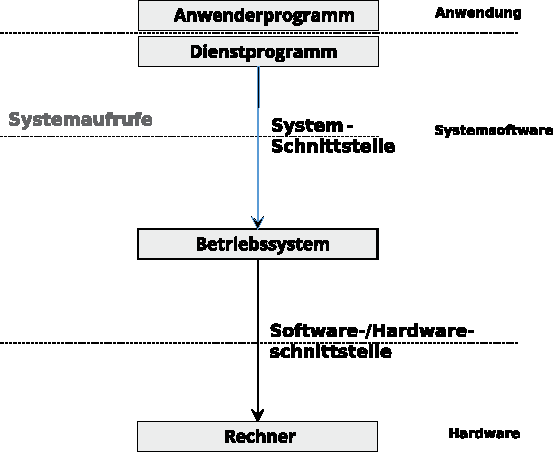
\includegraphics[]{images/betriebssysteme.pdf}
    \end{center}
\end{defi}

\begin{bonus}{Anforderungen an ein Betriebssystem}
    \begin{itemize}
        \item Hohe Zuverlässigkeit und Leistung
        \item Einfache Bedienbarkeit und Wartbarkeit
        \item Niedrige Kosten
    \end{itemize}
\end{bonus}

\begin{bonus}{Batchsysteme}
    \emph{Batchsysteme} sind dazu gedacht, Rechenaufgaben ohne Nutzereingabe abzuarbeiten.
    Dazu gibt es eine \emph{Job Queue}, in welche Aufgaben eingestellt werden.
    Diese Aufgaben werden dann bearbeitet und die Ergebnisse an den Nutzer ausgegeben.
\end{bonus}

\begin{bonus}{Dialogsysteme}
    \emph{Dialogsysteme} sind auf eine Interaktion mit dem Benutzer ausgelegt.
    Sie sind die wohl geläufigste Form von Betriebssystemen, da diese Form auf z.B. Desktop-Computern eingesetzt wird.

    Dialogsysteme werden noch einmal unterteilt in \emph{Single User}- und \emph{Multi-User-Systeme}.
\end{bonus}

\begin{bonus}{Echtzeitsysteme}
    \emph{Echtzeitsysteme} sind reaktive Systeme, die mit Hilfe von Sensoren Ereignisse registrieren und anhand von Aktoren darauf reagieren.
    Dabei ist die zeitliche Abfolge bzw. die Dauer der Ausführung von Interesse.
\end{bonus}

\subsection{Prozess}

\begin{defi}{Prozess}
    Ein \emph{Prozess} ist die Abstraktion eines in Ausführung befindelichen Programms.

    Er besteht aus den \emph{Programmbefehlen} und dem \emph{Prozesskontext}.

    Der \emph{Prozesskontext} besteht aus dem privaten Adressraum des Prozessors, geöffneten Streams und abhängigen Prozessen.
\end{defi}

\begin{defi}{Prozesszustände}
    \begin{center}
        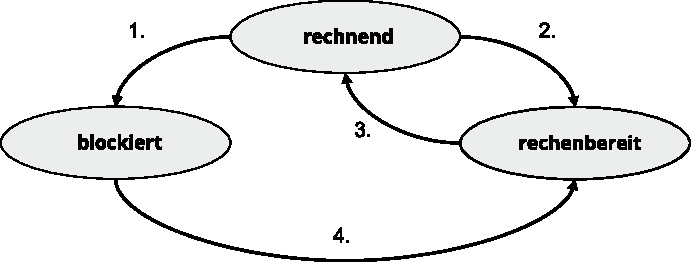
\includegraphics[]{images/prozesszustaende.pdf}
    \end{center}
    \begin{enumerate}
        \item Der Prozess muss auf ein externes Ereignis warten.
        \item Die Zeitscheibe des Prozesses ist abgelaufen, oder ein höher priorisierter Prozess muss ausgeführt werden.
        \item Der Prozess bekommt eine neue Zeitscheibe zugeteilt.
        \item Das externe Ereignis, auf das der Prozess gewartet hat, ist eingetreten.
    \end{enumerate}
\end{defi}

\begin{bonus}{Multitasking}
    \textbf{Preemptives Multitasking}:
    \begin{itemize}
        \item Betriebssystem entscheidet, wann welcher Prozess zur Ausführung kommt
        \item Benutzer erhält Eindruck von Parallelität
    \end{itemize}

    \textbf{Kooperatives Multitasking}:
    \begin{itemize}
        \item Prozess bestimmt selbst, wann er den Prozessor abgibt
        \item \emph{Nachteile}
              \subitem - z.B. Endlosschleifen können das gesamte System zum Absturz bringen
              \subitem - das Betriebssystem kann nicht berechnen, wann der Prozessor wieder frei ist
    \end{itemize}
\end{bonus}

\begin{defi}{Scheduling}
    Die Zuteilung von Zeitscheiben wird \emph{Scheduling} genannt und ist der Kern der Prozessverwaltung.
    Das Scheduling sollte dabei jederzeit die folgenden Eigenschaften erfüllen:
    \begin{itemize}
        \item \emph{Fairness}: Jeder Prozess erhält einen gerechten Anteil der CPU-Zeit.
        \item \emph{Effizienz}: Die CPU und andere Ressourcen sind möglichst vollständig ausgelastet.
    \end{itemize}
\end{defi}

\begin{bonus}{Priorität}
    \textbf{Statische Priorität}:
    \begin{itemize}
        \item Jeder Prozess erhält beim Start eine \emph{feste Priorität}
        \item Prozess mit \emph{höchster Priorität} bekommt als nächstes eine Zeitscheibe zugeteilt
        \item Oft in Echtzeitsystemen verwendet
    \end{itemize}

    \textbf{Dynamische Priorität}:
    \begin{itemize}
        \item Jeder Prozess erhält beim Start eine \emph{Anfangspriorität}
        \item Prozess mit \emph{höchster Priorität} bekommt als nächstes eine Zeitscheibe zugeteilt
        \item Prioritäten der Prozesse werden \emph{dynamisch geändert}
    \end{itemize}
\end{bonus}

\begin{algo}{Scheduling: FIFO (First In First Out)}
    Prozesse werden nach \emph{Reihenfolge} ihres Einfügens in die \emph{Job-Queue} bearbeitet.
    \begin{itemize}
        \item Zuteilung der CPU findet nur statt, wenn laufender Prozess wartet oder sich beendet
        \item Jeder Prozess kommt garantiert an die Reihe
        \item Kurze Prozesse müssen unter Umständen sehr lange warten, bis sie ausgeführt werden
    \end{itemize}
\end{algo}

\begin{algo}{Scheduling: SJF (Shortest Job First)}
    Prozesse werden aufsteigend nach ihrer \emph{geschätzten Ausführungszeit} bearbeitet.
    \begin{itemize}
        \item Große Prozesse kommen möglicherweise nie an die Reihe, wenn stets kleinere dazukommen
        \item Wartezeit auf das Ergebnis eines Prozesses sich in etwa proportional zur Ausführungszeit
    \end{itemize}
\end{algo}

\begin{algo}{Scheduling: MLFQ (Multilevel Feedback Queue)}
    Bei diesem Ansatz gibt \emph{mehrere FIFO-Queues}, denen jeweils
    eine \emph{Priorität} zugeordnet ist.

    Ein neuer Prozess wird immer in der Queue mit
    \emph{höchster Priorität} eingeordnet.

    Wird der Prozess während der ersten Zeitscheibe fertig,
    so verlässt er das System.

    Gibt er die CPU freiwillig ab, beispielsweise weil er
    durch das Warten auf ein externes Ereignis blockiert wird, wird er, sobald er wieder
    bereit ist, in \emph{dieselbe Queue wieder einsortiert} und dort weiter ausgeführt.

    Verbraucht der Prozess seine Zeitscheibe vollständig, so wird er in die \emph{nächst-niedriger priorisierte FIFO-Queue} eingereiht. Dort gelten wieder dieselben Regeln wie vorher.

    Verbraucht der Prozess immer weiter seine Zeitscheiben vollständig, kommt er
    schließich in der \emph{am niedrigsten priorisierten Queue} an.
    Dort verweilt er, bis er abgearbeitet wurde, d.h. es gibt \emph{keine Möglichkeit} wieder in höher priorisierte Queues
    eingestuft zu werden.

    Wieviele FIFO-Queues es gibt, ist vom konkreten Einsatzszenario abhängig.
\end{algo}

\subsection{Speicherverwaltung}

\begin{defi}{Reale Speicherverwaltung}
    Jedem Prozess wird ein zusammenhängener Block im Hauptspeicher zugeteilt.
    Wird in diesem Kontext der Arbeitsspeicher direkt aus den Prozessen heraus adressiert, spricht man von \emph{realer Speicherverwaltung}.

    Das bedeutet auch, dass die Größe des physikalisch vorhandenen Hauptspeichers die Anzahl der gleichzeitig ausführbaren Prozesse begrenzt.

    \emph{Nachteile}:
    \begin{itemize}
        \item Es muss Platz für das \emph{gesamte Programm und die Daten} gefunden werden.
        \item Es kannt nicht mehr Speicher genutzt werden, als \emph{physikalisch vorhanden}.
        \item Anforderung, zusammenhängender Speicherblöcke zu finden, verschärft Problem der \emph{Fragmentierung}.
    \end{itemize}
\end{defi}

\begin{bonus}{Fragmentierung}
    \emph{Fragmentierung} passiert dann, wenn mehrere, kleine Blöcke im Hauptspeicher frei sind und unter der Prämisse, dass einem
    Prozess ein zusammenhängender Block im Hauptspeicher zugeordnet werden
    muss, dies eventuell zu einer Situation führt, in der kein neuer Prozess gestartet
    werden kann, obwohl in Summe genügend Hauptspeicher frei wäre.
\end{bonus}

\begin{defi}{Swapping}
    Beim \emph{Swapping} wird der
    Hauptspeicherinhalt eines Prozesses auf den \emph{Hintergrundspeicher}, beispielsweise
    eine Festplatte (HDD), \emph{ausgelagert}, um Platz für andere Prozesse zu schaffen.

    Bekommt dann der Prozess, dessen Daten gerade auf dem Hintergrundspeicher liegen,
    die CPU zugeteilt, müssen seine Daten \emph{erneut in den Hauptspeicher geladen werden},
    wahrscheinlich nachdem die Daten eines anderen Prozesses ausgelagert wurden.
\end{defi}

\begin{defi}{Virtuelle Speicherverwaltung}
    Jedem Prozess wird ein \emph{scheinbar zusammenhängender Speicherbereich} zur Verfügung gestellt.
    Tatsächlich besteht der Speicher des Prozesses aus nicht zwangsläufig zusammenhängenden \emph{virtuelle Pages}.

    Der Prozess kann seinen Speicher mit \emph{virtuellen Adressen} beginnend bei 0 adressieren.

    Die Gesamtheit aller virtuellen Adressen wird als \emph{virtueller Adressraum} bezeichnet.
\end{defi}

\begin{defi}{Virtuelle Pages}
    \emph{Virtuelle Pages} werden auf Blöcke im Hauptspeicher gleicher Größe abgebildet.

    Hier kann auch \emph{Swapping} genutzt werden. In diesem Fall aber für einzelne Pages, nicht für den gesamten Hauptspeicherinhalt des Prozessors.
\end{defi}

\begin{defi}{Pagetable}
    Beim Zugriff auf eine virtuelle Speicheradresse durch einen Prozess muss diese
    Adresse in eine physikalische Adresse umgewandelt werden. Das geschieht anhand
    der \emph{Pagetable}, die das Betriebssystem \emph{für jeden Prozess} erstellt und aktualisiert.

    Da
    die Pagetable virtuelle Pages auf physikalische Pages gleicher Größe abbildet, gibt es einen Teil der Adresse, der sogenannte \emph{Offset}, der die Position der Daten innerhalb
    der Page angibt.

    Abhängig von
    der Größe der Pages besteht das Offset aus $m$ Bits.
    Für eine Pagegröße von 1MB
    werden beispielsweise 20 Bits als Offset benötigt.

    Der Rest der Adresse, die Seitennummer,
    muss dann anhand der Pagetable in die Basisadresse umgesetzt werden,
    um die Adresse im physikalischen Speicher zu erhalten. Da die Seitennummer aus
    $n$ Bits besteht, kann die Pagetable maximal $2^n$ Einträge enthalten.
\end{defi}

\begin{example}{Pagetable}
    Die Länge einer Adresse sei 16 Bit, aufgeteilt in je 8 Bit für Offset und Seitennummer.

    Es sei außerdem folgende Seitentabelle gegeben:

    \begin{center}
        \begin{tabular}{|c|c|c|}
            \hline
            \textbf{Eintrag} & \textbf{Gültig} & \textbf{Basisadresse} \\
            \hline
            00               & Nein            & -                     \\
            01               & Ja              & 0x17                  \\
            02               & Ja              & 0x20                  \\
            03               & Ja              & 0x08                  \\
            04               & Nein            & -                     \\
            05               & Ja              & 0x10                  \\
            \hline
        \end{tabular}
    \end{center}

    Dann können virtuelle Adressen anhand dieser Pagetable wie folgt umgesetzt werden:

    \begin{center}
        \begin{tabular}{|c|c|}
            \hline
            \textbf{virtuelle Adresse} & \textbf{physikalische Adresse}      \\
            \hline
            0x083A                     & ungültig (Seite 8 existiert nicht)  \\
            0x01FF                     & 0x17FF (Seite 1, Basisadresse 0x17) \\
            0x0505                     & 0x1005 (Seite 5, Basisadresse 0x10) \\
            0x043A                     & ungültig (Seite 4 ungültig)         \\
            \hline
        \end{tabular}
    \end{center}

    \emph{Hinweis}: Ist eine Adresse ungültig, wurde die dazugehörige Page in den Hintergrundspeicher ausgelagert. In diesem Fall muss die physikalische Page in den RAM geladen und die Pagetable aktualisiert werden.
\end{example}

\begin{bonus}{Paging on Demand}
    Das Vorgehen, aktuell
    unbenutzte Pages aus dem Hauptspeicher auf den Hintergrundspeicher auszulagern
    wird auch als \emph{Paging on Demand} bezeichnet.
    Das Ziel dabei ist, Arbeitsspeicher
    für andere Prozesse freizugeben.

    Dabei kann ein Prozess entweder Platz für eine
    bestimmte Anzahl von physikalischen Pages zugewiesen bekommen, die sich im
    Laufe der Prozessabarbeitung nicht ändert, oder es wird dynamisch anhand der aktuellen
    Speicherauslastung entschieden, wieviel Platz ein Prozess belegen darf.
\end{bonus}

\begin{algo}{Speicherverwaltung: FIFO (First In First Out)}
    Beim \emph{FIFO}-Verfahren wird
    diejenige Page ausgelagert, welche sich schon am längsten im Hauptspeicher
    befindet. Dazu muss in der Pagetable festgehalten werden, wann welche
    Page in den Hauptspeicher geladen wurde.
\end{algo}

\begin{algo}{Speicherverwaltung: LRU/LFU (Least Recently / Frequently Used)}
    Bei \emph{LRU}
    wird mitgehalten, wieviele Ladevorgänge seit der letzten Benutzung einer
    Page vorgenommen wurden. Das heißt, dass im Gegensatz zu FIFO, der
    Kontrollzustand bei der Verwendung einer Page wieder auf \glqq 0\grqq gesetzt wird.
\end{algo}

\begin{example}{Speicherverwaltung}
    Seitenanforderungen: 1, 2, 3, 4, 1, 2, 5, 1, 2, 3, 4, 5

    \textbf{FIFO-Strategie:}

    \begin{tabular}{|c|c|c|c|c|c|c|c|c|c|c|c|c|c|}
        \hline
        \multicolumn{1}{|c}{\textbf{Referenzfolge}} & \multicolumn{1}{c|}{} & 1                  & 2                  & 3                  & 4                  & 1                  & 2                  & 5                  & 1 & 2 & 3                  & 4                  & 5 \\
        \hline
        \hline
        \multirow{3}{*}{\textbf{Arbeitsspeicher}}   & Page 1                & \textcolor{red}{1} & 1                  & 1                  & \textcolor{red}{4} & 4                  & 4                  & \textcolor{red}{5} & 5 & 5 & 5                  & 5                  & 5 \\
                                                    & Page 2                &                    & \textcolor{red}{2} & 2                  & 2                  & \textcolor{red}{1} & 1                  & 1                  & 1 & 1 & \textcolor{red}{3} & 3                  & 3 \\
                                                    & Page 3                &                    &                    & \textcolor{red}{3} & 3                  & 3                  & \textcolor{red}{2} & 2                  & 2 & 2 & 2                  & \textcolor{red}{4} & 4 \\
        \hline
        \hline
        \multirow{3}{*}{\textbf{Kontrollzustand}}   & Page 1                & 0                  & 1                  & 2                  & 0                  & 1                  & 2                  & 0                  & 1 & 2 & 3                  & 4                  & 5 \\
                                                    & Page 2                & -                  & 0                  & 1                  & 2                  & 0                  & 1                  & 2                  & 3 & 4 & 0                  & 1                  & 2 \\
                                                    & Page 3                & -                  & -                  & 0                  & 1                  & 2                  & 0                  & 1                  & 2 & 3 & 4                  & 0                  & 1 \\
        \hline
    \end{tabular}

    9 Einlagerungen

    \textbf{LRU-Strategie:}

    \begin{tabular}{|c|c|c|c|c|c|c|c|c|c|c|c|c|c|}
        \hline
        \multicolumn{1}{|c}{\textbf{Referenzfolge}} & \multicolumn{1}{c|}{} & 1                  & 2                  & 3                  & 4                  & 1                  & 2                  & 5                  & 1 & 2 & 3                  & 4                  & 5                  \\
        \hline
        \hline
        \multirow{3}{*}{\textbf{Arbeitsspeicher}}   & Page 1                & \textcolor{red}{1} & 1                  & 1                  & \textcolor{red}{4} & 4                  & 4                  & \textcolor{red}{5} & 5 & 5 & \textcolor{red}{3} & 3                  & 3                  \\
                                                    & Page 2                &                    & \textcolor{red}{2} & 2                  & 2                  & \textcolor{red}{1} & 1                  & 1                  & 1 & 1 & 1                  & \textcolor{red}{4} & 4                  \\
                                                    & Page 3                &                    &                    & \textcolor{red}{3} & 3                  & 3                  & \textcolor{red}{2} & 2                  & 2 & 2 & 2                  & 2                  & \textcolor{red}{5} \\
        \hline
        \hline
        \multirow{3}{*}{\textbf{Kontrollzustand}}   & Page 1                & 0                  & 1                  & 2                  & 0                  & 1                  & 2                  & 0                  & 1 & 2 & 0                  & 1                  & 2                  \\
                                                    & Page 2                & -                  & 0                  & 1                  & 2                  & 0                  & 1                  & 2                  & 0 & 1 & 2                  & 0                  & 1                  \\
                                                    & Page 3                & -                  & -                  & 0                  & 1                  & 2                  & 0                  & 1                  & 2 & 0 & 1                  & 2                  & 0                  \\
        \hline
    \end{tabular}

    10 Einlagerungen
\end{example}

\newpage
\subsection{Dateisystemverwaltung}

\begin{defi}{BIOS (Basic Input/Output System)}
    Das \emph{BIOS}:
    \begin{itemize}
        \item ist die \emph{Firmware} bei x86-PCs
        \item liegt im \emph{nichtflüchtigen Speicher} auf der Hauptplatine des PCs
        \item leitet den \emph{Start} des \emph{Betriebssystems} ein
    \end{itemize}
\end{defi}

\begin{defi}{UEFI (Unified Extensible Firmware Interface)}
    \emph{UEFI} ist die zentrale Schnittstelle zwischen:
    \begin{itemize}
        \item der \emph{Firmware}
        \item den \emph{einzelnen Komponenten} eines Rechners
        \item und dem \emph{Betriebssystem}
    \end{itemize}
\end{defi}

\begin{bonus}{MBR (Master Boot Record)}
    Der \emph{MBR} besteht aus insgesamt 512 Byte, die sich auf 446 Byte
    für einen (optionalen) Bootloader, 64 Byte für die \emph{Partitionstabelle} und 2 Byte
    für eine \emph{} (0xAA55) aufteilen. Die Magic Number dient dazu, einen
    gültigen MBR zu identifizieren.

    In der Partitionstabelle können maximal 4 Partitionen
    definiert werden, d.h. die Festplatte kann in maximal 4 logische Einheiten aufgeteilt
    werden.
\end{bonus}

\begin{bonus}{GPT (GUID Partition Table)}
    Mit der Einführung von UEFI wurden auch die Limitierungen des
    MBR aufgehoben und die GPT als Nachfolger definiert.

    Die \emph{GPT} beinhaltet zu Beginn
    aus Kompatibilitätsgründen einen MBR, sodass ein hybrider Betrieb möglich
    ist. In der GPT können bis zu 128 Partitionen abgelegt werden.

    Zur Absicherung der
    GPT wird eine exakte Kopie der GPT am Ende des Datenträgers abgelegt.
\end{bonus}

\begin{defi}{Dateisystem}
    Ein Dateisystem ist im Prinzip eine Ablageorganisation für Daten auf einem Datenträger des Computers.
    Das Dateisystem muss sicherstellen,
    dass Dateien \emph{lesend und schreibend geöffnet} und auch wieder \emph{geschlossen} werden
    können. Das bedeutet, dass Dateinamen auf physikalische Adressen auf dem
    Datenträger abgebildet werden müssen.

    Spezielle Eigenschaften des Datenträgers
    (Festplatte, USB-Stick, ...) müssen berücksichtigt werden.

    Generell bieten
    alle (modernen) Dateisysteme folgende Attribute:
    \begin{itemize}
        \item Dateiname
        \item Ablageort (Ordner bzw. Verzeichnis)
        \item Dateigröße
        \item Zugriffsrecht
    \end{itemize}
\end{defi}

\begin{defi}{Lineare Dateisysteme}
    Bei linearen Dateisystemen werden Daten direkt hintereinander auf den Datenträger
    geschrieben. Das bedeutet, dass wahlfreier Zugriff nicht möglich ist. Daher finden
    diese Dateiysteme heutzutage nur noch Anwendung in Bereichen, in denen es nicht
    primär auf Geschwindigkeit ankommt.
\end{defi}

\begin{defi}{Hierarchische Dateisysteme}
    Daten werden auf hierarchischen Dateisystemen in einer Verzeichnisstruktur
    abgelegt.

    Diese Art von Dateisystem ist die wohl verbreiteste auf
    modernen Computern und kann auf Festplatten, SSDs, USB-Sticks, SD-Karten und
    sonstigen herkömmlichen Datenträgern verwendet werden.
\end{defi}

\begin{defi}{Netzwerkdateisysteme}
    In Netzwerkdateisystemen wird entfernter
    Speicher auf einem Server wie ein lokales Medium behandelt. Das Betriebssystem
    muss dann die Zugriffe auf Dateien in Netzwerkkommunikation umwandeln.
    Für den Nutzer
    eines Betriebsystems stellt sich Netzwerkspeicher allerdings in der Regel wie ein
    hierarchisches Dateisystem dar.
\end{defi}

\begin{bonus}{Sicherheitsaspekte}
    \textbf{Paralleler Zugriff im Multitasking}:
    \begin{itemize}
        \item Bereitstellung von Locks für den Dateizugriff
    \end{itemize}

    \textbf{Stromausfall während einer Schreiboperation}:
    \begin{itemize}
        \item Es muss Datenkonsistenz gewährleistet werden
        \item Atomare Operationen, welche entweder abgeschlossen oder ausstehend sind
              \subitem $\to$ Journalingdateisysteme
    \end{itemize}
\end{bonus}

\begin{defi}{Journalingdateisysteme}
    Bei einem Journalingdateisystem werden alle Aktionen auf der Festplatte protokolliert
    und erst als gültig aufgefasst, nachdem das Beenden der Aktion auf dem Dateisystem
    im \emph{Journal} (Protokoll) vermerkt wurde.

    \begin{itemize}
        \item \emph{Metadatenjournaling}:
              \subitem - Konsistenz des Dateisystems
        \item \emph{Fulljournaling}:
              \subitem - Konsistenz des Dateisystems
              \subitem - Konsistenz der Dateiinhalte
    \end{itemize}

\end{defi}

\section{Virtualisierung}

\begin{defi}{Virtualisierung}
    \emph{Virtualisierung} bezeichnet Methoden, die es erlauben, Ressourcen
    eines Computers \emph{zusammenzufassen oder aufzuteilen}.

    Dies wird erreicht, indem real existierende Hardware unter
    Zuhilfenahme einer Softwareschicht zu virtueller Hardware \emph{abstrahiert} wird.

    Dabei können mehrere Szenarien unterschieden werden:
    \begin{itemize}
        \item Partitionierung
        \item Aggregation
        \item Emulation
        \item Isolation
    \end{itemize}
    \vspace{1em}
    \begin{center}
        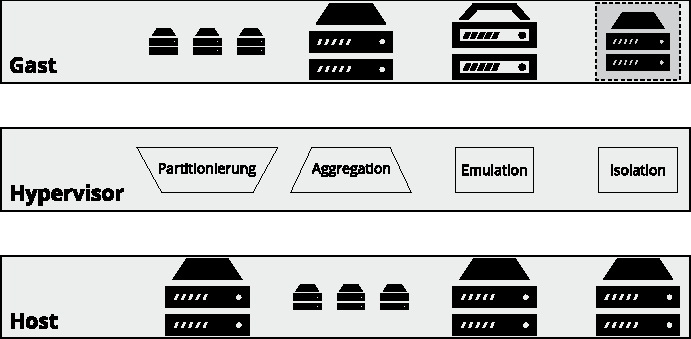
\includegraphics[]{images/virtualisierung.pdf}
    \end{center}
\end{defi}

\begin{defi}{Hypervisor / Virtual Machine Monitor (VMM)}
    Der \emph{Hypervisor} ist ein Stück Soft- oder Hardware, das  die Umsetzung
    zwischen der \emph{virtuellen Maschine} und der \emph{physikalischen Hardware} vornimmt.

    \textbf{Typ-1-Hypervisor}:
    \begin{itemize}
        \item läuft direkt auf physikalischer Hardware
    \end{itemize}

    \textbf{Typ-2-Hypervisor}:
    \begin{itemize}
        \item läuft als Anwendung auf dem Hostsystem
    \end{itemize}
\end{defi}

\subsection{Virtualisierungskonzepte}

\begin{defi}{Paravirtualisierung}
    \begin{itemize}
        \item Funktionalitäten des Gast BS werden gezielt verändert (Kernel Anpassungen)
        \item Gast-BS \glqq weiß\grqq, dass es sich in einer virtuellen Umgebung befindet
        \item Gast-BS kann direkt mit dem Hypervisor interagieren, benötigt keine Hardware-Emulation
    \end{itemize}

    \emph{Vorteile}: gute Performance

    \emph{Nachteile}: Gastsysteme nicht beliebig wählbar, hoher Aufwand für Kernel-Entwickler
\end{defi}

\begin{defi}{Hardware-unterstützte Virtualisierung}
    \begin{itemize}
        \item Neue Prozessortechnologien: CPUs besitzen Befehlssatz, der Virtualisierung unterstützt
        \item Modifikation des Gast-BS soll vermieden werden, direkt durch Hardware gelöst
        \item Hypervisor soll durch hardwarebasierte Speicherverwaltung entlastet werden
    \end{itemize}

    \emph{Vorteile}: Gast-BS muss nicht modifiziert werden, Gastsysteme frei wählbar

    \emph{Nachteile}: kein gemeinsamer Standard, Virtualisierungsplattform muss Technologie unterstützen
\end{defi}

\begin{defi}{Hardware-Emulation}
    \begin{itemize}
        \item Innerhalb einer VM wird Standardhardware eines Rechners komplett oder teilweise simuliert
        \item Emulator erzeugt Softwareschnittstellen, die vom Gast-BS angesprochen werden können
        \item Emulator sorgt dafür, dass Befehle, die an simulierte Hardware gerichtet sind, für die physische Hardware des Hostsystems umgewandelt werden
    \end{itemize}

    \emph{Vorteile}: flexible Wahl der Gast-BS

    \emph{Nachteile}: Performanceverlust durch hohen Virtualisierungsaufwand
\end{defi}

\begin{defi}{Betriebssystemvirtualisierung}
    \begin{itemize}
        \item Innerhalb des Host-BS werden Virtual Environments (VE) / Container erzeugt
        \item In VE ist kein eigenständiges Betriebssystem installiert
        \item Kernel-Bibliotheken und Geräte-Treiber des Hostsystems genutzt
        \item Einige Individualdaten müssen für Container definiert werden \\ (z.B. Dateisystem, IP Adresse, Hostname)
    \end{itemize}

    \emph{Vorteile}: gute Performance, wenig Speicherbedarf

    \emph{Nachteile}: keine freie Wahl des Gast-BS (gebunden an Hostsystem)
\end{defi}

\subsection{Cloud Computing}

\begin{defi}{Cloud Computing}
    \emph{Cloud Computing} ist im Wesentlichen ein Model um einen allgegenwärtigen,
    bequemen, bedarfsgesteuerten Netzwerkzugang zu einem gemeinsamen Pool konfigurierbarer
    Computer-Ressourcen zur Verfügung zu stellen. Zudem soll das Ganze
    schnell und mit minimalem Verwaltungsaufwand und Interaktion mit dem Provider
    funktionieren.
\end{defi}

\begin{defi}{Servicemodelle}
    \textbf{Infrastructure as a Service} (IaaS):
    \begin{itemize}
        \item vom Anbieter verwaltete Infrastruktur
        \item Nutzer muss verwendetes Betriebssystem und Software vollständig selbst verwalten
    \end{itemize}

    \textbf{Platform as a Service} (PaaS):
    \begin{itemize}
        \item virtuelle Plattform zur Verfügung gestellt (Betriebssystem, Entwicklungsplattform)
        \item alles \glqq unterhalb\grqq der Plattform ist aber \emph{nicht} unter der Kontrolle des Nutzers
    \end{itemize}

    \textbf{Software as a Service} (SaaS):
    \begin{itemize}
        \item nur eine einzelne Anwendung zur Verfügung gestellt
        \item alles \glqq unterhalb\grqq der Anwendung ist aber \emph{nicht} unter der Kontrolle des Nutzers
    \end{itemize}
\end{defi}

\begin{bonus}{Charakterisken von Cloud Computing}
    \begin{itemize}
        \item Selbstverwaltung (On-demand self-service)
        \item Breitband Internetzugang
        \item Ressourcenbündelung
        \item Elastizität
        \item Leistungsmessung
    \end{itemize}
\end{bonus}

\begin{defi}{Bereitstellungsmodelle}
    \textbf{Private Cloud}:
    \begin{itemize}
        \item für eine ganz spezielle Nutzergruppe betrieben
        \item kann auch von der Firma selbst verwaltet werden
    \end{itemize}

    \textbf{Community Cloud}:
    \begin{itemize}
        \item wird für verschiedene Nutzergruppen in einem bestimmten Kontext betrieben
        \item in der Regel von einer der teilnehmenden Gruppen oder von externem Dienstleister bereitgestellt
    \end{itemize}

    \textbf{Public Cloud}:
    \begin{itemize}
        \item für beliebige Nutzer zur Verfügung steht
        \item von beliebigem Anbieter betrieben
    \end{itemize}

    \textbf{Hybrid Cloud}:
    \begin{itemize}
        \item kombiniert mehrere der vorhergehenden Bereitstellungsmodelle
        \item einzelnen Teile unabhängig voneinander, aber durch standardisierte Schnittstellen verbunden
    \end{itemize}
\end{defi}

\section{Datenschutz und Sicherheit}
\subsection{Datensicherheit}

\begin{defi}{Kryptographie}
    Kryptographie ist die Wissenschaft der Verschlüsselung von Informationen. Sie wird genutzt
    um Informationen auf eine Art und Weise zu verändern, sodass ein Unbefugter
    die Informationen nicht mehr lesen kann. Es soll nur dem tatsächlichen Adressaten
    einer Nachricht möglich sein, diese auch zu lesen. Es geht also explizit nicht darum,
    den Diebstahl von Informationen zu verhindern, sondern es geht darum, dass
    entwendete Informationen nicht gelesen werden können.
\end{defi}

\begin{defi}{Transpositionschiffren}
    Die Verschlüsselung wird durch Umordnung der Zeichen
    im Klartext umgesetzt.
\end{defi}

\begin{defi}{Substitutionschiffren}
    Die Verschlüsselung wird durch Ersetzung der Zeichen
    im Klartext realisiert.

    \textbf{Monoalphabetische Substitution}:
    \begin{itemize}
        \item Jedes Zeichen des Klartexts wird durch genau
              ein eindeutiges Zeichen aus dem Geheimtextalphabet ersetzt, das für einen
              gewählten Schlüssel immer gleich ist.
    \end{itemize}

    \textbf{Homophone Substitution}:
    \begin{itemize}
        \item Jedes Zeichen des Klartexts wird durch genau ein
              anderes Zeichen aus einer eindeutigen Menge von Zeichen ersetzt, die für einen
              gewählten Schlüssel immer gleich ist.
    \end{itemize}

    \textbf{Polyalphabetische Substitution}:
    \begin{itemize}
        \item Jedes Zeichen wird durch ein eindeutiges Zeichen
              aus einem von mehreren geheimen Alphabeten ersetzt, die für einen gewählten
              Schlüssel immer gleich sind. Die Alphabete werden dabei immer der Reihe nach
              verwendet.
    \end{itemize}
\end{defi}

\begin{example}{Cäsar Chiffre}
    Im einfachsten Fall beinhalten $\mathfrak{P}$ und $\mathfrak{S}$ dieselben Zeichen und sind nur gegeneinander
    um $k$ Zeichen verschoben. Diese Variante einer \emph{monoalphabetischen Substitutionschiffre} wird \emph{Cäsar Chiffre} genannt.

    Alice wählt für die Verschlüsselung $k = 10$ und erhält damit die folgenden Alphabete:

    \begin{center}
        $\mathfrak{P}$: \texttt{A B C D E F G H I J K L M N O P Q R S T U V W X Y Z}\\
        $\mathfrak{S}$: \texttt{J K L M N O P Q R S T U V W X Y Z A B C D E F G H I}\\
    \end{center}

    Da Alice $k = 10$ gewählt hat, beginnt das Geheimtextalphabet mit \texttt{J}, dem
    zehnten Buchstaben des Alphabets. Die Verschlüsselung führt Alice durch,
    indem sie jeden Buchstaben ihres Klartexts durch den entsprechenden Buchstaben
    aus dem Geheimtextalphabet ersetzt.Werden die beiden Alphabete wie
    weiter oben aufgeschrieben, ist das einfach der Buchstabe im Geheimtextalphabet
    der direkt unter dem Buchstaben im Klartextalphabet steht. Damit ergibt
    sich für die Nachricht \texttt{HALLO} der Geheimtext \texttt{QJUUX}. Bob kann den
    Geheimtext dann entschlüsseln, indem er wiederum beide Alphabete untereinander
    schreibt und jedem Buchstaben aus dem Geheimtext den zugehörigen
    Buchstaben aus dem Klartextalphabet zuorndet, der dann genau darüber steht.
\end{example}

\begin{example}{Vigenère Chiffre}
    Eine bekannte \emph{polyalphabetische Substitutionschiffre} ist die \emph{Vigenère Chiffre}.
    Sie funktioniert im Prinzip wie die Cäsar-Chiffre, verwendet also verschobene
    lateinische Alphabete zur Verschlüsselung. Wie viele Alphabete und wie
    jedes von ihnen verschoben, wird durch den Schlüssel $k$ bestimmt, der in diesem
    Fall ein Wort ist. Es gibt also soviele geheime Alphabete, wie es Zeichen
    in $k$ gibt und jedes dieser Alphabete ist verschoben, so dass das $i$-te Alphabet
    mit dem $i$-ten Zeichen von $k$ beginnt.
    Alice wählt das Schlüsselwort $k = EDV$. Damit ergeben sich Klartext- und
    Geheimalphabete wie folgt:

    \begin{center}
        $\mathfrak{P}$: \texttt{A B C D E F G H I J K L M N O P Q R S T U V W X Y Z}\\
        $\mathfrak{S}_1$: \texttt{E F G H I J K L M N O P Q R S T U V W X Y Z A B C D}\\
        $\mathfrak{S}_2$: \texttt{D E F G H I J K L M N O P Q R S T U V W X Y Z A B C}\\
        $\mathfrak{S}_3$: \texttt{V W X Y Z A B C D E F G H I J K L M N O P Q R S T U}\\
    \end{center}

    Damit kann Alice den Klartext $M =$ \texttt{HALLOHALLO} verschlüsseln, indem Sie
    die Buchstaben des Klartexts wie bei der Cäsar Chiffre zuordnet und dabei die
    drei Geheimtextalphabete reihum verwendet. Da der Klartext mehr Zeichen
    enthält, als es Geheimtextalphabete gibt, fängt sie nach jeweils drei Zeichen
    wieder beim ersten Geheimtextalphabet an. Somit ergibt sich der Geheimtext
    $C =$ \texttt{LDGPRCEOGS}.
\end{example}

\begin{defi}{Moderne Verschlüsselungsverfahren}
    Moderne Verschlüsselungsverfahren werden, im Gegensatz zu klassischen Verfahren,
    nicht mehr auf Zeichen einer natürlichen Sprache angewandt. Stattdessen werden
    Zahlen bzw. Bits als Grundlage der Operationen verwendet. Damit können
    beliebige Daten verschlüsselt werden, nicht mehr nur Text. Damit sind moderne
    Verschlüsselungsverfahren den Anforderungen der heutigen digitalen Gesellschaft
    gewachsen.

    \textbf{Symmetrische Verfahren}:
    \begin{itemize}
        \item denselben Schlüssel zur Ver- und Entschlüsselung
        \item Problem des Schlüsselaustauschs
        \item Vertraulichkeit, aber keine zur Sicherstellung von Authentifizierung und Integrität
        \item[$\to$] Blockchiffren
            \subitem -  zu verschlüsselnde Daten in $m$ Blöcke derselben Größe aufgeteilt
            \subitem -  einfachster Fall: jeder der zuvor erzeugten Blöcke $m_i$ mit Schlüssel $k$
            \subitem zu verschlüsseltem Block $c_i$ derselben Größe übersetzt
        \item[$\to$] Stromchiffren
            \subitem -  Klartext wird bitweise anhand eines Schlüsselstroms verschlüsselt
            \subitem - Schlüsselstrom und Geheimtext haben dieselbe Länge wie der Klartext
    \end{itemize}

    \textbf{Asymmetrische Verfahren}:
    \begin{itemize}
        \item Die meisten asymmetrischen Verfahren basieren auf mathematischen Problemen, die nicht effizient zu lösen sind.
        \item
    \end{itemize}
\end{defi}

\begin{algo}{RSA Verschlüsselung}
    RSA basiert auf der Faktorisierung ganzes Zahlen, für die es keinen bekannten
    effizienten Algorithmus gibt. Dabei geht es darum, eine Zahl in ihre Primfaktoren
    zu zerlegen.

    Da beide Schlüssel des Schlüsselpaars zusammen funktionieren sollen, müssen sie
    nach einer festen Vorschrift erzeugt werden:
    \begin{enumerate}
        \item Wähle zwei Primzahlen $p, q$ mit $p \neq q$
        \item Berechne $N = p \cdot q$
        \item Berechne $\varphi(N) = (p-1)\cdot (q-1)$
        \item Wähle ein $e$, das teilerfremd zu $\varphi(N)$ ist mit $1 < e < \varphi(N)$
        \item Berechne $d$, sodass $e \cdot d \equiv 1 \mod \varphi(N)$
    \end{enumerate}

    Nach dieser Prozedur ist $(e,N)$ der \emph{public key} und $(d,N)$ der \emph{private Key}. Damit
    kann nun jeder Nachricht $M \in \N, 1 < M < N$ anhand folgender Formel verschlüsselt
    werden:
    $$
        C = M^e \mod N
    $$

    Die Entschlüsselung der verschlüsselten Nachricht $C$ kann dann anhand einer ähnlichen Formel durchgeführt werden:
    $$
        M = C^d \mod N
    $$
\end{algo}

\begin{example}{RSA Verschlüsselung}
    Damit Alice Bob eine Nachricht schreiben kann, muss Bob zunächst seinen \emph{public Key} zur Vefügung stellen.

    Zur Erzeugung seines Schlüsselpaars wählt Bob die Primzahlen $p=13$ und $q=17$.
    Damit ergibt sich $N = 221$ und $\varphi(N) = 192$.
    Anschließend wählt Bob $e=5$ und berechnet damit $d=77$.
    Damit kann Bob $(5, 221)$ als seinen \emph{public Key} an Alice geben und $(77, 221)$ behält er als \emph{private Key} für sich.

    Alice hat nun Bobs \emph{public Key} und möchte damit die Nachricht $M = 42$ verschlüsseln.
    Dazu berechnet Sie $C = 42^5 \mod 221 = 9$ und schickt die verschlüsselte Nachricht anschließend an Bob.

    Bob kann nun mit seinem \emph{private Key} die erhaltene Nachricht entschlüsseln und erhält $M = 9^77 \mod 221 = 42$.
\end{example}

\begin{defi}{Digitale Signatur}
    Um auch \emph{Authentifizierung}
    und \emph{Integritat} herstellen zu können, muss eine digitale Signatur verwendet
    werden. Dazu braucht es zunachst eine \emph{Hashfunktion}, die eine Art Fingerabdruck
    der Nachricht erzeugt.

    Nachdem mit der Hashfunktion der Hashwert der Nachricht berechnet wurde, wird
    dieser mit dem \emph{private Key} des Senders verschlüsselt.

    Danach berechnet
    der Empfänger selbst den Hashwert der empfangen Nachricht. Stimmen der
    selbst berechnete Hashwert und der entschlüsselte Hashwert überein ist die \emph{Integrität} der Nachricht sichergestellt. Da zudem das Entschlüsseln des Hashwertes mit
    dem öffentlichen Schlüssel des Senders funktioniert hat, ist der Sender authentifiziert,
    da dessen privater Schlüssel zur Erstellung der digitalen Signatur verwendet
    wurde.

    Es ist also notwendig, dass sich Sender und Empfanger vorab auf eine
    Hashfunktion einigen. Zusatzlich ist wichtig zu beachten, dass eine Digitale Signatur
    \emph{keine Vertraulichkeit} herstellt, dazu muss die Nachricht zusatzlich verschlüsselt
    werden.
\end{defi}

\begin{defi}{Hybride Chiffren}
    Die Kombination von symmetrischen und asymmetrischen
    Chiffren nennt man \emph{hybride Chiffren}.

    \begin{itemize}
        \item verhältnismäßig kurzer Schlüssel einer Blockchiffre wird asymmetrisch verschlüsselt und zum Empfänger einer Nachricht transportiert
        \item Kommunikation selbst läuft symmetrisch verschlüsselt ab
        \item Kombination erzielt guten Kompromiss zwischen Sicherheit und Rechenaufwand
    \end{itemize}
\end{defi}

\printindex
\printindex[Beispiele]
\end{document}
